\chapter{Arquitectura y Diseño}
\label{Arquitectura}

VirtShell Framework es un API REST diseñado para simplificar la automatización y gestión de infraestructura, facilitando tareas como creación, despliegue y mantenimiento de recursos virtuales. Para lograr esto, VirtShell se basa en scripts de shell re-utilizables, que permiten instalar y configurar cualquier tipo de servidor o grandes soluciones que involucren varios recursos virtuales sin importar su tamaño. VirtShell es un framework de código abierto y bajo la licencia BSD, que permite utilizarlo para proyectos de cualquier tipo, incluso comerciales. \\
\\
\section{Características}

\begin{description}
\item [Programable] VirtShell esta principalmente orientado a realizar el aprovisionamiento de sus instancias en scripts de shell permitiendo aprovechar todas las estructuras y utilidades del lenguaje de programacion. Adicionalmente VirtShell permite extender el comportamiento del shell desplegando comandos propios que proporcionan ahorro en tiempo y en complejidad. Sin embargo, el lenguaje de shell no es de uso obligatorio, el  metodo de aprovisionamiento puede ser el de la preferencia del usuario. 
\item [Repetible] VirtShell ofrece herramientas para que los scritps de aprovisionamiento sean configurables y que puedan ser ejecutados varias veces en diferentes ambientes de desarrollo o produccion.
\item [Modular] VirtShell es un framework organizado de forma modular. Los modulos se encuentran agrupados en categorias que ofrecen las herramientas necesarias para la administracion de y aprovisionamiento de multiples recursos virtuales.
\item [Seguro] VirtShell provee varias capacidades y servicios para aumentar la privacidad y el control de acceso a los diferentes recursos. Los servicios de seguridad permiten crear redes y controlar el acceso a las instancias creadas, asi como definir y administrar politicas de accesso a usuarios y permisos sobre cualquier recurso del sistema como por ejemplo scripts de creacion y aprovisionamiento.
\item [Extensible] VirtShell fue diseñado con la idea de cargar codigo dinamicamente facilmente, permitiendo extender el comportamiento del framework agregando plugins en tiempo de ejecucion.
\item [Inyección de dependencias virtuales] VirtShell adopta la idea del patrón de Inyección de Dependencias, para conseguir scripts de aprovisionamiento mas desacoplados, facilitando a un recurso virtual configurar las dependencias que tiene de otras máquinas virtuales para realizar su trabajo. Para ello, el framework permiten declarar el listado de dependencias de recursos virtuales que tiene un script aprovisionamiento permitiendo el correcto acople entre los diferentes recursos virtuales. 
\end{description}

\section{Arquitectura}
VirtShell Framework consiste de caracteristicas organizadas en 12 modulos. Estos modulos son agrupados en Seguridad, Administracion y Aprovisionamiento. Estos elementos se usan de manera separada pero trabajan juntos para proveer la informacion necesaria para que los agentes realicen su trabajo en los hosts que albergaran los recursos virtuales, como se muestra en la figura. \\

\begin{figure}
	\caption{Overview of the VirtShell Framework}
	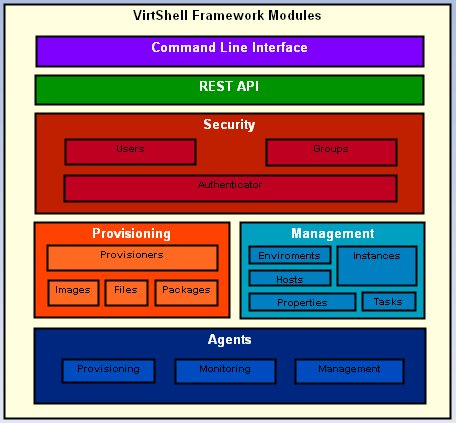
\includegraphics[width = 0.75\textwidth]{figures/framework}
\end{figure}

Las siguientes secciones detallan los módulos disponibles para cada característica. 

\subsection{Security}
El modulo de seguridad consisten en los modulos de usuarios, grupos y el modulo de autenticacion. El control de los usuarios y grupos es un elemento clave en la administración del framework.\\
\\
Los Usuarios pueden ser personas reales, es decir, cuentas ligadas a un usuario físico en particular o cuentas que existen para ser usadas por aplicaciones específicas.\\
\\
Los Grupos son expresiones lógicas de organización, reuniendo usuarios para un propósito común. Los usuarios dentro de un mismo grupo pueden leer, escribir o ejecutar los recursos que pertenecen a ese grupo.\\
\\
El modulo de autenticación soporta el proceso por el cual cuando un usuario se presenta a la aplicación puede validar su identidad es, de hecho, quien decide si tiene permiso para ingresar al sistema y el nivel de acceso a un recurso dado. En el capitulo 4 se detalla el proceso de autenticacion y autorizacion.

\subsection{Managment}



\subsection{Provisioning}

\subsection{Agents}


